\documentclass[12pt]{article}
\usepackage{a4wide}
\usepackage[utf8]{inputenc}
\usepackage{mathtools}
\usepackage{amssymb}
\usepackage[english]{babel}
\usepackage{mdframed}
\usepackage{systeme,}
\usepackage{lipsum}
\usepackage{relsize}
\usepackage{caption}
\usepackage{tikz}
\usepackage{tikz-3dplot}
\usepackage{pgfplots}
\usepackage{harpoon}%
\usepackage{graphicx}
\usepackage{wrapfig}
\usepackage{subcaption}
\usepackage{authblk}
\usepackage{float}
\usepackage{listings}
\usepackage{xcolor}
\usepackage{amsmath}
\usepackage{chngcntr}
\usepackage{amsthm}
\usepackage{comment}
\usepackage{commath}
\usepackage{hyperref}%Might remove, adds link to each reference
\usepackage{url}
\newcommand{\w}{\omega}
\newcommand{\curl}[1]{\mathbf{\nabla}\times \mathbf{#1}}
\newcommand{\grad}{\mathbf{\nabla}}
\newcommand{\dive}[1]{\mathbf{\nabla}\cdot \mathbf{#1}}
%\newcommand{\crr}{\mathfrak{r}}
\usepackage{calligra}

\DeclareMathAlphabet{\mathcalligra}{T1}{calligra}{m}{n}
\DeclareFontShape{T1}{calligra}{m}{n}{<->s*[2.2]callig15}{}
\newcommand{\crr}{\mathcalligra{r}\,}
\newcommand{\boldscriptr}{\pmb{\mathcalligra{r}}\,}
\newcommand{\res}[2]{\text{Res}(#1,#2)}
\newcommand{\G}{\mathcal{G}}
\newcommand{\note}{\textit{Note: }}
\newcommand*{\colorboxed}{}
\def\colorboxed#1#{%
  \colorboxedAux{#1}%
}
\newcommand*{\colorboxedAux}[3]{%
  % #1: optional argument for color model
  % #2: color specification
  % #3: formula
  \begingroup
    \colorlet{cb@saved}{.}%
    \color#1{#2}%
    \boxed{%
      \color{cb@saved}%
      #3%
    }%
  \endgroup
}

\title{Mathematical Methods: FK7048}
\author{Author: Andreas Evensen}
\date{Date: \today}
\definecolor{codegreen}{rgb}{0,0.6,0}
\definecolor{codegray}{rgb}{0.5,0.5,0.5}
\definecolor{codepurple}{rgb}{0.58,0,0.82}
\definecolor{backcolour}{rgb}{0.95,0.95,0.92}

\lstdefinestyle{mystyle}{
    backgroundcolor=\color{backcolour},   
    commentstyle=\color{codegreen},
    keywordstyle=\color{magenta},
    numberstyle=\tiny\color{codegray},
    stringstyle=\color{codepurple},
    basicstyle=\ttfamily\footnotesize,
    breakatwhitespace=false,         
    breaklines=true,                 
    captionpos=b,                    
    keepspaces=true,                 
    numbers=left,                    
    numbersep=5pt,                  
    showspaces=false,                
    showstringspaces=false,
    showtabs=false,                  
    tabsize=2
}

\lstset{style=mystyle}

\begin{document}

\maketitle
\begin{figure}[H]
    \centering
    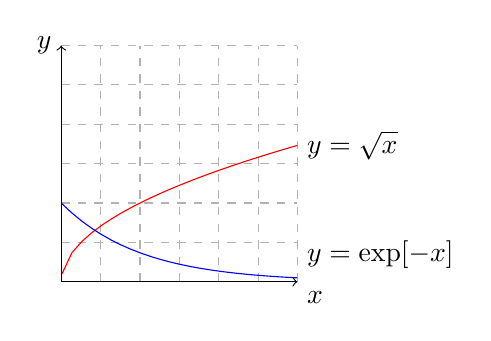
\begin{tikzpicture}
        \draw[dashed, black!30, step = 0.5] (0,0) grid (3,3); 
        \draw[red, thin, domain = 0.01:3] plot(\x, {sqrt(\x)}) node[right] {\color{black} $y = \sqrt{x}$};
        \draw[blue, thin, domain = 0.01:3] plot(\x, {exp(-\x)}) node[anchor = south west] {\color{black} $y = \exp[-x]$};
        \draw[->, black] (0,0) -- (3,0) node[anchor = north west] {  $x$};
        \draw[->, black] (0,0) -- (0,3) node[anchor = east] {$y$};
    \end{tikzpicture}
\end{figure}
\newpage
\tableofcontents
\newpage

\section{Ordinary Differential Equations}
In this course, one covers four different types of Ordinary Differential equations: Seperable first order differential equations, Exact differentail equations, Homogenous differential equations, and linear differential equations; all of them are first order differential equations. The general form of any order differential equation is:
\begin{align*}
    \sum_{i = 1}^n a_{n-i}\frac{d^{n-i}}{x^{n - i}}y(x) = 0.
\end{align*}
\noindent
The following sections cover the different types of differential equations, and how to solve them. This will be for the general first order ode, written on the form:
\begin{align}
    a_1(x)\cdot y'(x) = f(x,y)\label{eq: first order general case}
\end{align}

\subsection{Seperable ODE's}
Seperable ODEs are ODE's that can be seperated into two sets of functions:
\begin{align*}
    y'(x) = f(x,y) = \frac{P(x,y)}{Q(x,y)}
\end{align*}In the case of $P$ and $Q$ being seperable, one means that both can be written explicitly as a function of $x$ or $y$, i.e. $P(x)$ and $Q(y)$ or vice versa.
In that case, one can write the following:
\begin{align*}
    Q(y)dy = P(x)dx, \text{ or } \frac{dy}{P(y)} = \frac{dx}{Q(x)}.
\end{align*}One can then integrate both sides and solve for $y$ as a function of $x$; \textit{Note:} when integrating, one has to use reference integration, i.e. form $y_0$ to $y$ and $x_0$ to $x$.
\subsection{Exact ODE's}
Suppose that $f(x,y)$ can't be written as two seperate functions only depending on a single variable, but rather as a function of both $x$ and $y$:
\begin{align*}
    \frac{dy}{dx} = f(x,y) = \frac{P(x.y)}{Q(x,y)},
\end{align*}then one can write it on the following form:
\begin{align*}
    P(x,y)dx + Q(x,y)dy = 0.
\end{align*}Using the fact that mixed derivatives are equal one can solve this problem as a three-step method:
\begin{align*}
    \frac{\partial \psi}{\partial y} = Q(x,y) \quad \& \quad \frac{\partial \psi}{\partial x} = P(x,y),
\end{align*}for an arbitrary function $\psi(x,y)$.
\begin{itemize}
    \item Evaluate, if true then we proceed, and it might be possible to solve via this method: $$\frac{\partial Q}{\partial x} = \frac{\partial P}{\partial y} = \frac{\partial^2 \psi}{\partial x\partial y}$$
    \item Evaluate: $$\frac{\partial \psi}{\partial x} = P(x,y).$$ Don't miss any integration constant or functions of $y$.
    \item Evaluate: \begin{align*}
        &Q(x,y)dy + P(x,y)dx = 0\\
        &\implies \int \frac{\partial \psi}{\partial y}dy + \int \frac{\partial \psi}{\partial x}dx = c\\
        &\implies \psi(x,y) = \frac{c}{2}
    \end{align*}
\end{itemize}It might not be possible to write it on an explicit form, but rather an implicit form, i.e. $F(x,y) = c$.

\subsection{Homogenous ODE's}
In this case, one does not mean that the $f(x,y)$ term in the general case \eqref{eq: first order general case} is $0$ but rather the following:
\begin{align*}
    f(kx, ky) = k^n \cdot f(x,y).
\end{align*}In order tos solve this type of ODE, one use the following:
\begin{align*}
    &Q(x,y)dy + P(x,y)dx = 0\\
    \implies & xQ^*(x,v)dv + [P^*(x,v) + v]dx= 0 \\
    \implies & xP^*(v)dv + Q^*(v)dx = 0\\
    \implies & \frac{P^*(v)}{Q^*(v)}dv = \frac{1}{x}dx
\end{align*}\note the variable change. An example of this is the following:
\begin{align*}
    &\frac{dy}{dx} = -\frac{x}{x + y}\\
    \implies& (x+y)dy + xdx = 0\quad [y = xv]\\
    \implies &(x + xv)(xdv + vdx) + xdx = 0\\
    \implies & x(x+ v)dv = -(v + v^2+ 1)dx.
\end{align*}And form this point it's trivial to solve. The entire point of this method is to make the ODE seperable, but in order to do so, a clever subsitution is required.

\subsection{Linear ODE's}
Linear ODE's have the following form:
\begin{align*}
    \colorboxed{red}{\frac{dy}{dx} + p(x)y = q(x).}
\end{align*}These are solved via the so called integrating factor:
\begin{align*}
    &\alpha(x) = \exp\left[\int p(x)dx\right]\\
    \implies& y(x) = \int \frac{\alpha(x)q(x) - c}{\alpha(x)}dx
\end{align*}An example of this would be the ODE $y'(x) + 2y = 2e^{2x}$:
\begin{align*}
    a(x)&=\int p(x)dx = exp\left[\int 2dx\right] = e^{2x}\\
    y(x) &= \int \frac{\alpha(x)q(x) - c}{\alpha(x)}dx\\
    &= \int \frac{e^{2x}2e^{2x} -c}{e^{2x}}dx\\
    &=\frac{1}{2}e^{2x}+ c_1 e^{-2x} + c_2.
\end{align*}Using boundary conditions one then finds the two integration constants.

\subsection{Solving higer order ODE's}
Higher ODE's can be harder to solve, but a good way to start is by making the ansats $y(x)=e^{rx}$ and find the roots of the characteristic equation; this is only possible when the ODE has constant coefficients, i.e.
that the constants infront of the terms is indenpendent of $x$. If the root are real and distinct, then the solution is given by, for a second order problem:
\begin{align*}
    y(x) = Ae^{r_1x} + Be^{r_2x}.
\end{align*}However, if the roots are the same, we instead get:
\begin{align*}
    y(x) = Ae^{r_1x} + xBe^{r_1x}.
\end{align*}If the problem is inhomgenous, i.e. that it's source-function $f(x)\neq 0$, then the total solution is given by particular solution added to the homogenous solution, i.e. $y(x) = y_p(x) + y_h(x)$.
From here it's important to note that there exists something called singularity points; where the functions $p(x)$ and/or $q(x)$ diverges.
\begin{itemize}
    \item \textbf{Regular singular points}: where $p(x)$ and $q(x)$ approaches $\infty$, but where $(x-x_0)p(x)$ and $(x-x_0)^2q(x)$ don't.
    \item \textbf{Regular singular points}: where $p(x)$ and $q(x)$ approaches $\infty$, but where $(x-x_0)p(x)$ and $(x-x_0)^2q(x)$ also does.
\end{itemize}

\subsection{Power series solutions}
There exists two methods of solving via a power-series ansats, either the power-series ansats or the Frobenius anstats.
\begin{align}
    \text{Frobenius: }& \colorboxed{red}{y(x) = \sum_{n = 0}^\infty a_n x^{n + r}},\label{eq: Frobenius ansats}\\
    \text{Power series: }&\colorboxed{red}{y(x) = \sum_{n = 0}^\infty a_n x^{n}}.\label{eq: Power series ansats}
\end{align}The method of this is to differentiate the expressions twice, reindex to find write everything on same exponent, and then find the recursion relation. In doing so,
one can compare them to Taylor-expansions and find the corresponding functions. In the case of the Frobenius ansats, one has to find the indicial equation, is the $n = 0$ term of the expansion: the roots of the 
indicial equation, which are used to substitute the unknown $r$ in the series-expansion.
\subsection{Finding additional solutions}
Suppose that one finds one of the solutions to a problem, such that $y(x) = y_1(x) + y_2(x)$, then one can use Abel's theorem to find the second solution:
\begin{align*}
    y_2(x) = k y_1(x) \int \left(\frac{\exp\left[-\int_{x_0}^x p(\w)d\w\right]}{\big(y_1(x)\big)^2}dx\right),
\end{align*}where $k$ is an arbitrary constant. This is only valid for linear ODE's. But also, the Wronskian of two solutions is given by:
\begin{align*}
    W(y_1,y_2) &= k\exp\left[\int_{x_0}^x p(\w)d\w\right]\\
    &= \begin{vmatrix}
        y_1 & y_2\\
        y_1' & y_2'
    \end{vmatrix} = y_1y_2' - y_2y_1'.
\end{align*}If the Wronskian is zero, then the two solutions are linearly dependent, and one can't use Abel's theorem to find the second solution.
\subsubsection{Variation of parameters}
Suppose we have the following:
\begin{align*}
    y''(x) + p(x)y'(x) + q(x)y(x) = F(x).
\end{align*}Finding the particular solution can be done via the methods above, however the particular solution can also be stated to have the following form:
\begin{align*}
    y_p(x) = A_1(x)y_1(x) + A_2(x)y_2(x),
\end{align*}where $y_i(x)$ are the solutions to the homogneous problem, and $A_i(x)$ are unknown functions. These functions can be found via the following:
\begin{align*}
    &A_1'(x)y_1'(x) + A_2'(x)y_2'(x) = F(x),\\
    \implies& \colorboxed{red}{A_1(x) = \int -\frac{1}{W(y_1,y_2)}y_2(x)F(x)dx},\\
    \implies& \colorboxed{red}{A_2(x) = \int \frac{1}{W(y_1,y_2)}y_1(x)F(x)dx},\\
\end{align*}where $W$ is the Wronskian.
\section{Storm-Louiville equation}
Suppose an ODE on the following form:
\begin{align}
    \frac{d}{dx}\left[p(x)\frac{dy}{dx}\right] + [q(x)+\lambda r(x)]y = 0,\label{eq: SL}
\end{align}the function $r(x)$ is called the weighting function and is defined as:
\begin{align*}
    \int_a^b r(x)y_n(x)y_m(x)dx = \delta_{nm},
\end{align*}where $y_i(x)$ are the eigenfunctions of the problem. When doing SL problems, one finds that the solutions are eigenfunctions. Moreover, if $\lambda$ in eq \eqref{eq: SL} is equal to zero, then the problem becomes self-adjoint.
That is the following:
\begin{align}
    \colorboxed{red}{\frac{d}{dx}\left[p(x)\frac{dy}{dx}\right] + q(x)y = 0,}\label{eq: self-adjoint SL}
\end{align}
\subsection{Bondary conditions}
There exists a few classifications on boundary conditions:
\begin{itemize}
    \item \textbf{Dirichlet}: $y(a) = y(b) = 0$.
    \item \textbf{Neumann}: $y'(a) = y'(b) = 0$.
    \item \textbf{Robin}: $y'(a) = 0$ and $y(b) = 0$.
\end{itemize}In this list above, all the boundary conditions are homogenous, however that does not have to be the case; they can also be non-homogenous, i.e. that they are non-zero: a function or a constant.

\subsection{Converting an ODE into SL form}
Many ODEs' can be converted into SL form using the following method:
\begin{align*}
    &p_0(x)\psi'' + p_1(x)\psi' + p_2(x)\psi = \lambda \psi\\
    &w(x)= \frac{1}{p_0(x)}\exp\left[\int \frac{p_1(x)}{p_0(x)}dx\right]\\
    \implies \lambda \psi w(x) &= w(x)\left(p_0(x)\psi'' + p_1(x)\psi' + p_2(x)\psi\right)\\
    \implies& \bar{p}_0' = \frac{d}{dx}\exp\left[\frac{p_0}{p_0}\int\frac{p_1}{p_0}dx\right]=\bar{p}_1
\end{align*}$\bar{p}_0$ is now the first term of the expansion, which is the weighing-function times the original-expression, and the second term is computed in accordance to the above expression. An example of this would be the following:
\begin{align*}
    &xy'' + (1-x)y' + 1 = 0\\
    w(x)&= \frac{1}{x}\exp[\int\frac{1-x}{x}dx] = e^{-x}
\end{align*}

\section{Partial Differential Equations}
There exists mulitple different types of ordinary differential equations, however in this course only linear PDEs' were covered and those being that of: Hyperbolic-, Parabolic-, and Elliptic- PDEs'. A second order PDE is defined as the following:
\begin{align}
    A(x,y)f_{xx} + 2B(x,y)f_{xy} + C(x,y)f_{yy} + D(x,y)f_x + E(x,y)f_y + F(x,y)f = G(x,y).\label{eq: general PDE of second order}
\end{align}We compute the different types of PDE's in accordance to the list below:
\begin{itemize}
    \item \textbf{Hyperbolic}: $B^2 - AC > 0$.
    \item \textbf{Elliplitc}: $B^2 - AC < 0$ 
    \item \textbf{Parabolic}: $B^2 - AC = 0$.
\end{itemize}The different types of PDEs' have different behaviors, and different methods of solving them. The following sections will cover the different types of PDEs' and how to solve them.
\subsection{Different common PDE's}
The Laplace-equation, eq \eqref{eq: Laplace-equation} is defined below and is an example of an elliptic PDE:
\begin{itemize}
    \item \textbf{Laplace-equation}: \begin{align}
    \Delta f(x,y,z) = \nabla^2 f(x,y,z) = 0.\label{eq: Laplace-equation}
\end{align}This is obviously a second order PDE, but since $B = 0$ given the general case eq \eqref{eq: general PDE of second order} it's an elliptic equaption.
    \item \textbf{Poission-equation}: \begin{align}\Delta f(x,y,z) = \nabla^2 f(x,y,z) = -\frac{\rho}{\epsilon_0}.\label{eq: Poission-equation}\end{align}This is also an elliptic PDE.
    \item \textbf{Heat-equation}: \begin{align*}\nabla^2f = \frac{1}{a^2}\frac{\partial f}{\partial t}\end{align*}This is also an elliptic PDE.
    \item \textbf{Wave-equation}:\begin{align*}
    \nabla^2f = \frac{1}{c^2}\frac{\partial^2 f}{\partial t^2}
\end{align*}This is also an elliptic PDE.
    \item \textbf{Schrödingers-equation}:\begin{align*}
    -\frac{1}{\hbar m}\nabla^2 \psi+ V\psi = i\hbar\frac{\partial \psi}{\partial t}
\end{align*}
    \item \textbf{Klein Gordons-equation}: \begin{align*}
    &\square\psi = -\mu^2\psi\\
    \square &= \frac{1}{c^2}\frac{\partial^2}{\partial t^2} - \nabla^2
\end{align*}
\end{itemize}
\subsection{Solving PDE's}
There exists numerous ways of solving PDE's, however most PDE's are solved via the aid of computers via methods such as: \underline{method of lines}. However, there exists a few methods for solving PDE's by hand: Seperation of variables, Fourier transforms \ref{sec: fourier transform}, 
method of characteristic and so on. This section is divided such that they cover each of the different methods covered in this course.
\subsubsection{Method of characteristic}
Suppose a first order PDE on the following form:
\begin{align*}
    A(x,y)u_x + B(x,y)u_y + C(x,y)u = D(x,y).
\end{align*}Suppose the case when $A$ and $B$ are constants and the others are zero:
\begin{align*}
    &au_x+ bu_y = 0.\\
    \implies & [a,b]\cdot\begin{pmatrix}
        \frac{\partial}{\partial x}\\
        \frac{\partial }{\partial y}
    \end{pmatrix}u
\end{align*}Using some clever change of variable: $s = ax + by$ and $t = bx - ay$ one can solve this problem. The method of characteristic is a method of solving first order PDE's, and is done by the following:
\begin{align*}
    &\frac{\partial u}{\partial s} = 0\\
    &\frac{\partial u}{\partial t} = u(t)
\end{align*}An example of this would be:
\begin{align*}
    3u_x + 4u_y = 0\quad \&\quad u(0,y) = \sin(y).
\end{align*}This is then written on the following form:
\begin{align*}
    (3,4)\cdot\begin{pmatrix}
        \frac{\partial}{\partial x}\\
        \frac{\partial }{\partial y}
    \end{pmatrix}u
\end{align*}Using the variable change: $s = 3x + 4y$ and $t = 4x - 3y$ one has that:
\begin{align*}
    &u(t) = u(4x - 3y)\\
    &u(0,y) = \sin(y)\implies u(x,y) = \sin\left(4y -3x\right)
\end{align*}In the cases where $A$ and $B$ are not constants but rather functions one instead has:
\begin{align*}
        &A(x,y)u_x+ B(x,y)u_y = 0.\\
    \implies & [A(x,y),B(x,y)]\cdot\begin{pmatrix}
        \frac{\partial}{\partial x}\\
        \frac{\partial }{\partial y}
    \end{pmatrix}u
\end{align*}This instead yields characteristic curves, and the solution is given by:
\begin{align*}
    \frac{dy}{dx} = \frac{B(x,y)}{A(x,y)}.
\end{align*}There also exists a plug and play variant of this solution method: Suppose that one has the following PDE:
\begin{align*}
    A(x,y)u_x + B(x,y)u_y = C(x,y).
\end{align*}Then the solution can be found via the following, which is called the \textbf{Lagrange-Charpit Equation}:
\begin{align}
    \colorboxed{red}{\frac{dx}{A(x,y,z)} = \frac{dy}{B(x,y,z)} = \frac{dz}{C(x,y,z)}}\label{eq: Lagrange-Charpit Equation}
\end{align}Note this method only works for first order PDE's, and if the variables are non-coupled. If they are coupled, one has to de-couple them first by taking the derivatives multiple times to get rid of the coupling.

\subsubsection{Seperation of variables}
Some PDE's can be solved using the method of seperation of variables; which effectivly takes and PDE to and ODE; this is a very powerful technique which takes the form:
\begin{align*}
    u(x,y) = X(x)Y(y).
\end{align*}This is then inserted into the PDE and using an example one would get the following, the Laplace-equation \eqref{eq: Laplace-equation}:
\begin{align*}
    &u_{xx} + u_{yy} = 0\\
    \implies & \frac{X''(x)}{X(x)} + \frac{Y''(y)}{Y(y)} = 0\\
    \implies& \frac{X''}{X} = -\frac{Y''}{Y} = \lambda^2
\end{align*}This means that the rate of change is the same, which is just some constant, thus one can write the following:
\begin{align*}
    u(x,y) = X(x)Y(y) = \left(c_1e^{-\lambda x} + c_2e^{\lambda x}\right)\cdot\left(c_3\sin(\lambda y) + c_4\cos(\lambda y)\right)
\end{align*}\note many of the PDE's in time are evaluated in the so-called \textit{steady state}, i.e. that the time-derivative is zero, e.g. that the system has reached an equalibrium. Also, not every system is seperable; it puts constraints on the system.
\subsection{Notes}
The Hessian of a system:
\begin{align*}
    H = \begin{vmatrix}
        \frac{\partial^2}{\partial x^2} & \frac{\partial^2}{\partial x\partial y} & \frac{\partial^2}{\partial x\partial z}\\
        \frac{\partial^2}{\partial x\partial y}& \frac{\partial^2}{\partial y^2}& \frac{\partial^2}{\partial y\partial z}\\
        \frac{\partial^2}{\partial x\partial z}& \frac{\partial^2}{\partial y\partial z}& \frac{\partial^2}{\partial z^2}
    \end{vmatrix}
\end{align*}If the eigenvalues of the Hessian $H$ are positive and real, then there exists a local minimum, if it's negative and real, then there exists a local maximum and if it's zero then there exists a saddle-point.
\section{Green's Functions}
Green's function are a way to solve ordinary differnetial equations, and can be used to solve partial differnetial equations however that is not covered in this course. These functions are defined as the solution to the following equation:
\begin{align}
    &\frac{d}{dx}\left[p(x)\frac{dy}{dx}\right] + q(x)y(x) = f(x),\label{eq: greens-function}\\
    &\mathcal{L}G(x,x') = \delta(x - x')\nonumber,
\end{align}where $\mathcal{L}$ is a linear operator defined by the problem at hand. One solves the two set of equations:
\begin{align*}
    &\G_1(s,s) = \G_2(s,s), \text{ Continuity condition}\\
    &\frac{d\G_2}{dx}(x,s)\Bigg|_{x = s} - \frac{d\G}{dx}(xs)\Bigg|_{x = s} = \frac{1}{p(x)}.\text{ Discontinuity condition}
\end{align*}Green's functions are used to solve inhomogenous differential equations on the form \eqref{eq: greens-function}. And the solution is given in totalt to be:
\begin{align*}
    &\colorboxed{red}{y(x) = \int_0^x \G_1(x,s)f(s)ds + \int_{x}^L\G_2(x,s)f(s)ds},\\
    &\colorboxed{red}{\G(x,s) = \begin{cases}
        \G_1(x,s), & 0\leq s\leq x,\\
        \G_2(x,s), & x\leq L.
    \end{cases}}
\end{align*}\textbf{Are they swapped?}

\section{Complex Analysis}
A complex number $z$ can be defined as $z = a + bi$ or $z(x,y) = u(x,y) + i (v,y)$. In doing so, one finds that the differentiability of such a function $z$ would be the following:
\begin{align*}
    \colorboxed{red}{\frac{\partial u }{\partial x} = \frac{\partial v}{\partial y}\quad \&\quad \frac{\partial u}{\partial y} = - \frac{\partial v}{\partial x},}
\end{align*}which is also known as the Cauchy-Riemann equations. The laplacian $\nabla^2$ in the complex space is a bit more tricky and is defined by:
\begin{align*}
    \colorboxed{red}{\frac{\partial^2 u }{\partial x^2} + \frac{\partial u}{\partial v^2} = \frac{\partial^2 v}{\partial y\partial x} - \frac{\partial^2v}{\partial x\partial y} = 0.}
\end{align*}
If the function $z$ is differentiable, then it is also analytic. A function $f(z)$ can be analytic around points: singularities. 
There exists two kinds of singularities: essential-singularities and poles. Essential singularities are when the function $f(z)$ diverges fast enough to be expanded into a Laurent series.
\begin{align}
    f(z) &= \sum_{n = -\infty}^\infty a_n(z - z_0)^n.\label{eq: laurent-expansion}\\
    a_n &= \frac{1}{2\pi i}\oint_C \frac{f(\tilde{z})}{(\tilde{z} -z_0)^{n+1}} d\tilde{z} \nonumber
\end{align}The $a_{-1}$ coefficient is known as the residue of the function $f(z)$. \textit{Note:} a good trick so solving problems in complex is via a change of coordinates, from cartesian to polar on euler form, i.e. $z = x + iy = re^{i\theta}$.

\subsection{Residue}
The residue is important when computing complex contour integrals:
\begin{align*}
    \colorboxed{red}{\oint_{\partial \Gamma} f(z)dz = 2\pi i \sum_{i} \res{f}{z_i},}
\end{align*}where $\Gamma$ is the closed contour and $z_i$ are the singularities of the function $f(z)$; note not essential-singularities, but rather poles of different order. There exists three ways to compute the residue of a function $f(z)$: Finding the Laurent series, or the following two methods:
\begin{align}
    &\colorboxed{red}{\res{f}{z_i} = \lim_{z\to z_i} (z - z_i)f(z),\label{eq:res1}}\\
    &\colorboxed{red}{\res{f}{z_i} = \lim_{z\to z_i}\frac{1}{(n-1)!} \frac{d^{(n-1)}}{dz^{(n-1)}}(z - z_i)^nf(z).\label{eq:res2}}
\end{align} In eq \eqref{eq:res1} one can compute the residue of a simple pole, and in eq \eqref{eq:res2} one can compute the residue of a pole of order $n$. An important trick is to deconstruct the function $f$ such that one can find the Taylor/Mclaren-series of each component, and then find the residue of the $(z - z_0)^{-1}$ term.
Also, if one tries to use eq \eqref{eq:res1} and one gets $\infty$ the reason it's because it's a higher order pole and one should use eq \eqref{eq:res2} instead. 
\subsection{Contour Integral tricks}
Suppose one has a funciton $f$ which is analytic expect at a point $z_0$, and one wants to compute the ingral, one can decompose the closed integral to the elements along a certain path $\Gamma$ and the elements around the point $z_0$:
\begin{align*}
    \oint_{\partial \gamma} f(z)dz &= 2\pi i \res{f}{z_0}\\
    &=\sum_{i}\int_{\Gamma_i} f(z)dz.
\end{align*}Often, the decomposed integrals might be easier to compute than the original integral, or maybe one of the integrals is the one that is wanted. Moreover, Cauchy's integral formula states the following:
\begin{align*}
    \text{Cauchy's integral formula: }
    &\colorboxed{red}{f(z_0)=\frac{1}{2\pi i}\oint_\Gamma \frac{f(z)}{z - z_0}dz },\\
    &\colorboxed{blue}{f^{n}(z_0) = \frac{n!}{2\pi i}\oint_{\Gamma} \frac{f(z)}{(z-z_0)^{n+1}}dz}
\end{align*}where $z_0$ is a singularity point. An example of the usefullness of this could be the following:
\begin{align*}
    &\oint_\Gamma \frac{\sin^2(z)}{(z-a)^4}dz\\
    \implies& f(z) = \sin^2(z)\\
    \implies& \oint_\Gamma \frac{\sin^2(z)}{(z-a)^4}dz = \frac{2\pi i}{3!}f^{(3)}(z = a)
\end{align*}

\subsection{Moreras Theorem}
Moreras theorem is equvilent to the fundamental theorem of calculus, but in the complex plane. It states the following: {\color{blue} If there exists a contionous function $f(z)$ on a simply connected in some region $\Gamma$, then}:
\begin{align*}
    \colorboxed{blue}{\oint_{\Gamma}f(z)dz = 0,}
\end{align*}{\color{blue} then $f(z)$ is analytic everywhere in $\Gamma$.} The implication of this is that $F'(z) = \frac{F(z_1) - F(z_0)}{z_1 - z_0}$ which is equvilent to the fundamental theorem of calculus.

\subsection{Branch cut}
When doing complex integration one can stumble upon a distinct problem, that a function is not properly defined for a certain value; or that it's not unqiuely defined. A common example is the function $f(z) = \ln(z)\cdot g(z)$, where $\ln(z)$ is, in a complex sense, not symemtric. The function $f(z)$ can only be solved with a branch-cut, i.e. that the contour is defined in a specific manner. Suppose the following integral, where $p\in(0,1)$:
\begin{align*}
    I = \int_0^\infty \frac{x^p}{x^2 + 1}dx.
\end{align*}Turning this integral to the complex plane one would have the following:
\begin{align*}
    \oint_\Gamma \frac{z^p}{z^2 + 1}dz.
\end{align*}However, there exists a problem; we have a branch-cut at $z = 0$ since $z^p = r^p e^{2i\pi p}$. One thus have to do the following analysis:
\begin{align*}
    \oint_\Gamma \frac{z^p}{z^2 + 1}dz &= \int_{\partial\Gamma_1} \frac{r^p}{r^2 + 1}dz + \int_{\partial\Gamma_2} \frac{z^p}{z^2 + 1}dz + \int_{\partial \Gamma_3} \frac{(re^{i2\pi})}{z^2 + 1}dz + \int_{\delta r}\frac{z^p}{z^2 + 1}dz\\
\end{align*}One sees that the integral over $\partial \Gamma_1$ is the integral one wants, but also $\partial\Gamma_3$ is the same with a phaseshift. Thus, one can compute the integral as the following:
\begin{align*}
    (1-e^{2\pi i p})I &= \oint_{\Gamma}\frac{z^p}{z^2 + 1} = 2\pi i\sum_{i}\res{f}{z_i},\\
    \implies I &= \frac{1}{1-  e^{2\pi ip}}\sum_{i}\res{f}{z_i}.
\end{align*}From this point, the only thing left is to compute the residues of the function $f(z)$, and since both are poles of the first kind one can use eq \eqref{eq:res1} to compute the residues.
\note when computing around a branch-cut, we avoid the essential-singuarlity by constructing a countour that avoids the point in itself.

\vspace{0.5cm}\noindent
Suppose that one has two functions $f$ and $g$ which are defined to be analytic on two domains $U_1$ and $U_2$ respectivly. If at the intersection there exists atleast one \textbf{accumulation point}, $ U = U_1\cap U_2$, one has that $f(z) = g(z)$, then one can define the following function:
\begin{align*}
    h(z) = \begin{cases}
        f(z); \forall z\in U_1\\
        g(z); \forall z\in U_2\cap U_1^C
    \end{cases}
\end{align*}where $U_1^C$ is the compliment domain. The Laruent expansion of the two functions are then defined as:
\begin{align*}
    f(z) &= \sum_{n = -\infty}^\infty a_n(z - z_0)^n\\
    g(z) &= \sum_{n = -\infty}^\infty b_n(z - z_1)^n
\end{align*}Then at the point accumulation point the following holds for all $n$:
\begin{align*}
    a_n(z-z_0)^n &= b_n(z-z_1)^n\\
    \implies \psi(z) = f(z) - g(z) &= \sum_{n = -\infty}^\infty (a_n - b_n)(z - z_0)^n = 0.
\end{align*}
\subsection{Cauchys principal value}
This is a method of given values to undetermined integrals which does not necessarily converge. Suppose that one has the following integral:
\begin{align*}
    \int_{-\infty}^\infty f(x)dx &= \lim_{R\to\infty}\int_{-R}^R f(x)dx\\
    &= \lim_{R\to\infty} F(x)\Bigg|_{x = -R}^R
\end{align*}An example of this could be the following:
\begin{align*}
    I &= \int_{0}^\infty \frac{\sin(x)}{x}dx = \int_0^\infty \frac{e^{ix} - e^{-ix}}{2ix}dx\\
    &= \int_0^\infty \frac{e^{ix}}{2ix}dx - \int_{0}^{\infty}\frac{e^{-ix}}{2ix}dx\\
    &= \int_0^\infty \frac{e^{ix}}{2ix}dx + \int_{-\infty}^{0}\frac{e^{ix}}{2ix}dx\\
    &= \int_{-\infty}^\infty \frac{e^{ix}}{2ix}dx
\end{align*}Using the complex integral of the same expression one can compute the value of the original expression:
\begin{align*}
    \lim_{R\to\infty}\oint_{\Gamma(R)}\frac{1}{2i}\frac{e^{iz}}{z}dz&= \int_{0}^\pi \frac{1}{2i}\frac{re^{i\theta}}{re^{i\theta}}d\theta +  \int_{\pi}^{2\pi} \frac{1}{2i}\frac{re^{i\theta}}{re^{i\theta}}d\theta = \pi.
\end{align*}Thus, the integral one first wanted is equal to half of that i.e. $I = \frac{\pi}{2}$.

\subsection{Meromorphic functions \& Winding numbers}
A function $f(z)$ is said to meromorphic at any point $z_0$ forall $z$ in the close neighbourhood of $z_0$ if the function can be decomposed as the following:
\begin{align*}
    f(z) = \frac{g(z)}{h(z)}.
\end{align*}If the two functions $g$ and $h$ are analytic at the point $z_0$ then the function $f$ is said to meromorphic around $z_0$. Another way to define it is to say that $h$ can only be $0$ at countable points. Meromorphic functions can be written as a 'non-infinite' Laruent series:
\begin{align*}
    f(z) =  \sum_{n = -N}^\infty a_n(z-z_0)^n.
\end{align*}This result is used in the \textbf{Mittag-Leffler theorem}. The theorem states: Assuming a function $f$ which is analaytic around the origin and only has countable singularities, $N$ in total, which are simple poles at $z_i$ with residues $a_i$, then the function $f$ can be written as the following:
\begin{align*}
    \colorboxed{red}{f(z) = f(0) + \sum_{i = 1}^Nb_i \left(\frac{z_i}{z - z_i} + \frac{1}{z_i}\right)}.
\end{align*}For this to hold the function $f$ has to be bounded, that is $f(z)\leq M$ for a constant $M$ in the contour that encompases all singularities. 

\vspace*{0.5cm}\noindent
\textbf{Winding numbers} are defined in laymans terms of how many times the function curls around itself. Assuming a function $f(z)$ which is analytic in some region $\Omega$ and a closed contour $\Gamma$ in $\Omega$ which does not pass through any singularities of $f(z)$, then the winding number is defined as:
\begin{align*}
    \colorboxed{blue}{\oint_\Gamma \frac{f'(z)}{f(z)}dz = 2\pi i w_n,}
\end{align*}where $w_n$ is the winding number. Now it should be identified that the winding-number $w_n$ is the sum of the residues, i.e. $w_n = \sum_i \res{f}{z_i}$ of the function in the integrand of the contour integral. This connects to \textbf{Rouche's theorem} which states: If $\Gamma$ is a closed contour and both the functions $f(z)$ and $g(z)$ are analytic inside and on $\Gamma$, and $|f(z)| > |g(z)|$ on $\Gamma$, then $f(z)$ and $f(z) + g(z)$ have the same number of zeros inside $\Gamma$.

\section{Bessel functions}
There exists multiple different kinds of Bessel-functions. Bessel-functions are solutions to the Bessel differential equation and often occur in problems with cylindrical symmetri:
\begin{align}
    \colorboxed{red}{x^2y'' + xy' + (x^2 - n^2)y = 0.}\label{eq: Bessel-equation}
\end{align}The term $n$ in the above equation is the so-called order of the equation, not to be confused with the order of the ODE. Bessel functions of the first kind are defined as:
\begin{align*}
    \colorboxed{red}{J_n(x) =\sum_{s = 0}^\infty \frac{(-1)^s}{s!(s + n)!}\left(\frac{x}{2}\right)^{2s + n}.}
\end{align*}They are found by solving the Bessel-equation, eq \eqref{eq: Bessel-equation} with either a power-series solution or a Frobenius solution.
One important property of Bessel functions is that they are orthogonal:
\begin{align*}
    \int_0^1 xJ_n(\lambda_{n,m}x)J_n(\lambda_{n,l}x)dx = \frac{1}{2}\delta_{m,l},
\end{align*}moreover, they have the following property, excluding the $n = 0$ case:
\begin{align*}
    J_{n+ 1}(x) - J_{n - 1}(x) &= 2J_n'(x),\\
    J_{n + 1}(x) + J_{n - 1}(x) &= \frac{2n}{x}J_n(x).
\end{align*}
The moddified Bessel functions are the Bessel-function with imaginary argument, i.e. the moddified Bessel-function of the first kind is defined as the following:
\begin{align*}
    \mathcal{J}_n(ix) = \sum_{k = 1}^\infty \frac{(-1)^k}{k!\Gamma(k + n + 1)}\cdot\left(\frac{ix}{2}\right)^{2k - n}
\end{align*}
\noindent
The integral representation of the Bessel-function of the first kind allows for easier computation of the expression of $J_n(x)$:
\begin{align*}
    J_n(x) =\frac{1}{\pi}\int_0^\pi\cos\left(n\tau - x\sin(\tau)\right)d\tau = \frac{1}{2\pi}\int_{-\pi}^\pi \exp\left[i(n\tau- x\sin(\tau))\right]d\tau,
\end{align*}and for the zeroth order Bessel-function one has the following:
\begin{align*}
    J_0(x) = \frac{1}{\pi}\int_0^\pi\cos\left(x\sin(\tau)\right)d\tau.
\end{align*}

\subsection{Legendre's polynomials}
The Legendre poylynomials, and the associate Legendre polynomials are solutions to the Legendre differential equation:
\begin{align}
    (1-x^2)\frac{d^2}{dx^2}P^m_l(x) - 2x\frac{d}{dx}P^m_l(x) + \left[l(l + 1) - \frac{m^2}{1 - x^2}\right]P^m_l(x) = 0.\label{Legendre equation}
\end{align}\note in this course, $m$ has been set to zero when solving the above equation, and thus is written on the following form:
\begin{align*}
   (1-x^2)p''(x) -2xy'(x) + l(l+1)p(x) = 0. 
\end{align*}
This equation is solved by the Legendre polynomials which can be derived from Rodrigues' formula:
\begin{align*}
    L_l(x) = \frac{1}{2^ll!}\frac{d^l}{dx^l}(x^2-1)^l,
\end{align*}which then gives the following solution to the associated polynomial:
\begin{align*}
    \colorboxed{red}{P^m_l(x) = (-1)^m(1 - x^2)^{m/2}\frac{d^m}{dx^m}P_l(x)}
\end{align*}
\subsection{Generating functions}
To solve certain problems one uses the concept of generating functions to solve the problem at hand; there exist multiple different generating functions however, the following is a known one:
\begin{align*}
    \colorboxed{blue}{g(x,t) = \frac{1}{\sqrt{1-2xt + t^2}} = \sum_{n = 0}^\infty P_n(x)t^n.}
\end{align*}

\subsection{Other special functions}
There exists other special functions, such as the Hermite polynomials, the Laguerre polynomials, and the Chebyshev polynomials. These will not be covered in this recap sheet. However, special functions such as the Gamma function, the Beta function and the Di-Gamma and Poly-Gamma functions can be defined in the following manner:

\begin{center}
    The Gamma-function $\Gamma$.
\end{center}
\begin{align*}
    \Gamma(z) &= \int_0^\infty t^{z - 1}e^{-t}dt,\\
    \Gamma(z)&= (z - 1)!\text{ if }z\in\mathbb{N}\\
    \text{Identity: }& \Gamma(z + 1) = z\Gamma(z),\\
    \text{Reflection: }& \Gamma(z + 1)\Gamma(1-z) = \frac{\pi}{\sin(\pi z)},\\
\end{align*}
\begin{center}
    The beta-function $\beta$.
\end{center}
\begin{align*}
    \beta(z, \w) &= \int_0^1 t^{z - 1}(1 - t)^{\w - 1}dt,\\
    &= \frac{\Gamma(z)\Gamma(\w)}{\Gamma(z + \w)} \text{ if z \& $\w$ are integers}\\
\end{align*}
\begin{center}
    The Di-Gamma function $\psi$.
\end{center}
\begin{align*}
    \colorboxed{red}{\psi(z) =\frac{d}{dz}\left(\ln(z)\right) = \frac{\Gamma'(z)}{\Gamma(z)}}
\end{align*}

\section{Transforms}
There exists numerous transforms, however in the course only linear transforms were considered; the transforms of Laplace and Fourier were taught. Both being linear operators. 
There exists other linear transforms, such as the Mellin transform, the Hankel transform, the Hilbert transform, the Z-transform, and the Radon transform. However, these will not be covered in this recap sheet.

\subsection{Fourier Transform}\label{sec: fourier transform}
The Fourier transform is defined as the operator $\mathcal{L}$ operating on a function $f(t)$ to be the $\tilde{f}(\w) = \mathcal{L}\big(f(t)\big)(\w)$. This is then defined as:
\begin{align*}
    \text{Transform: }\colorboxed{red}{\tilde{f}(\w) = \int_{-\infty}^\infty f(t)e^{-i\w t}dt,}\\
    \text{Inverse: }\colorboxed{red}{\quad f(t) = \frac{1}{2\pi}\int_{-\infty}^\infty \tilde{f}(\w)e^{i\w t}d\w.}
\end{align*}In order for the Fourier transform to exist, the function $f(t)$ must be absolutely integrable, i.e. $\int_{-\infty}^\infty |f(t)|dt < \infty$; moreover, the function $f$ has to be in $\mathbb{L}^1$. The transform has the following properties:
\begin{align}
    \text{1: }& \frac{df}{dx} \implies iw\tilde{f}(\w),\label{eq: Fourier derivative}\\
    \text{2: }& \frac{d^n f}{dx^n} \implies (iw)^n\tilde{f}(\w),\nonumber\\
    \text{3: }& (f \otimes g)(t) \implies \tilde{f}\cdot\tilde{g},\nonumber\\
    \text{4: }& f(at) \implies \frac{1}{|a|}\tilde{f}\left(\frac{\w}{a}\right),\nonumber\\
\end{align}An example of the Fourier transform is the $\chi$ function:
\begin{align*}
    \chi(-1,1) &= \begin{cases}
        1, & |x| < 1,\\
        0, &\text{elsewhere}
    \end{cases}\\
    \tilde{\chi}(\w) &= \int_{-1}^1 e^{-i\w t}dt = \frac{2\sin(\w)}{\w}.
\end{align*}

\subsection{Laplace Transform}
Another transform is the Laplace transform, $\hat{f}(s) = \mathcal{L}(f(t))(s)$, which is defined as:
\begin{align*}
    \hat{f}(s) &= \int_0^\infty f(t)e^{-st}dt\\
    f(t) &= \frac{1}{2\pi i}\lim_{T \to\infty}\int_{\gamma - iT}^{\gamma + iT} f(s)e^{st}ds,
\end{align*}where $\gamma$ is the real part of $s$. The Laplace transform has the following properties:
\begin{align*}
    \text{1: }& f'(t)\implies s\hat{f}(s) - \hat{f}(0^+),\\
    \text{2: }& f(t)\cdot t^{-1}\implies \int_{s}^\infty \hat{f}(x)dx,\\
    \text{3: }& f(t)e^{at}\implies \hat{f}(s-a),\\
    \text{4: }& f(at)\implies \frac{1}{\abs{a}}\hat{f}\left(\frac{s}{a}\right),\\
    \text{5: }& tf(t)\implies -\frac{d}{ds}\hat{f}(s).\\
\end{align*}The Laplace transform is a linear operator, and is defined for $t \geq 0$; since it's a linear operator, $\mathcal{L}(f + g)(s) = \hat{f} + \hat{g}$, and multiplication by a constant can be taken outside the operator.

\section{Usefull identifies}
\begin{align*}
    &\colorboxed{red}{\Gamma\left(\frac{1}{2}\right) = \sqrt{\pi}}\\
    &\colorboxed{blue}{n! = \frac{(2n)!!}{2^n}}\\
    &\text{Euler-Mascheroni constant: }\gamma = 0.5772...\\
\end{align*}
\newpage
\section{Practice Exam}

\subsection*{Problem 1)}
Solve the ODE:
\begin{align*}
    y'' + 4y = e^{x}; \quad y(0) = y'(0) = \frac{2}{5}.
\end{align*}

\subsubsection*{Solution}
Making the ansats $y = e^{rx}$ gives the characteristic equation:
\begin{align*}
    &e^{rx}(r^2 + 4) = 0 \implies r = \pm 2i.\\
    \implies& y_h(x) = a\cos(2x) + b\sin(2x).
\end{align*}The particular solution can be found by the method of undetermined coefficients:
\begin{align*}
    y_p(x) = Ae^x \implies y_p'(x) = Ae^x \implies y_p''(x) = Ae^x.
\end{align*}Substituting into the ODE gives:
\begin{align*}
    Ae^x + 4Ae^x = e^x \implies A = \frac{1}{5}.
\end{align*}Thus, the general solution is:
\begin{align*}
    y(x) = a\cos(2x) + b\sin(2x) + \frac{1}{5}e^x.
\end{align*}Applying the initial conditions gives:
\begin{align*}
    y(0) = a + \frac{1}{5} = \frac{2}{5} \implies a = \frac{1}{5}\\
    y'(0) = -2b + \frac{1}{5} = \frac{2}{5} \implies b = -\frac{1}{10}.
\end{align*}Thus, the solution is:
\begin{align*}
    y(x) = \frac{1}{5}\cos(2x) - \frac{1}{10}\sin(2x) + \frac{1}{5}e^x.
\end{align*}

\subsection*{Problem 2)}
Explain/Sketch-out (in a few equations and sentences) the following methods for solving 1st Ordinary ODEs:
\begin{enumerate}
    \item Seperation of variables
    \item Exact differential equations
    \item Homogeneous ODEs
    \item Linear ODE's
\end{enumerate}

\subsubsection*{Solution}
\begin{enumerate}
    \item \textbf{Seperation of variables}: Assuming a form $\frac{dy}{dx} = \frac{p(x,y)}{q(x,y)}$ where one only depends on one variable, then moving to either side and integrate.  
    \item \textbf{Exact differential equations}: Is a first order ODE where $\frac{dy}{dx} = f(x,y) = \frac{g(x,y)}{h(x,y)}$. In exact differential equations, neither $g$ nor $h$ can be written as a function of only one variable and thus one has to construct the following $\psi_y = g$ and $\psi_x = h$ and then solve the ODE $\frac{d\psi}{dx} = h$.
    \item \textbf{Homogeneous ODEs}: This type of ODE does not refer to the source-function being $0$ but rather the type of ODE where the function can be written on the followig form $f(kx,ky)=k^nf(x,y)$. Solving such a system one makes a variable substitution and solves the system with the transformed variables.
    \item \textbf{Linear ODEs}: This type of ODE has the following form: $y' + p(x)y = q(x)$, where $p(x)$ and $q(x)$ are functions of $x$. This type of ODE can be solved by the method of integrating factors, where one multiplies the ODE by the integrating factor $\alpha(x) = e^{\int p(x)dx}$.
\end{enumerate}

\subsection*{Problem 3)}
Show that:
\begin{align*}
    (1-x^2)y'' -xy' +n^2y = 0,
\end{align*}can be but put on SL-from with the following substitution: $\sqrt{(1-x^2)}$. Also, explain the orthangonaility condition of the SL problem under the transformation.

\subsubsection*{Solution}
There exists more than one way of doing this, one would be to compute the weighting-function; if the weighting is the same as the suggested transformation then the transformation is valid; another way would be to plug it into the equation by multiplying both sides by the transform:
However, in this instance the weighting-function option is opted:
\begin{align*}
    w(x) &= \frac{1}{1-x^2}\exp\left[\int \frac{-x}{1-x^2}dx\right]\\
    &= \frac{1}{1-x^2}\exp\left[\frac{\ln(x^2 -1)}{2}\right] = \frac{\sqrt{x^2 -1}}{1-x^2}\\
\end{align*}

\subsection*{Problem 4)}
Solve via the method of Frobenius:
\begin{align*}
    x^2y'' -2xy' +y = 0.
\end{align*}

\subsubsection*{Solution}
Ansats, centered around $x = 0$:
\begin{align*}
    y(x) &= \sum_{n = 0}^\infty a_n x^{n + r},\\
    y'(x) &= \sum_{n = 0}^\infty a_n(n+r) x^{n + r - 1},\\
    y''(x) &= \sum_{n = 0}^\infty a_n(n+r)(n+r-1) x^{n + r - 2}.
\end{align*}Substiting this into the ode yields:
\begin{align*}
    &x^2\sum_{n = 0}^\infty a_n(n+r)(n+r-1) x^{n + r - 2} - 2x \sum_{n = 0}^\infty a_n(n+r) x^{n + r - 1} + \sum_{n = 0}^\infty a_n x^{n + r} = 0\\
    &\sum_{n = 0}^\infty a_n(n+r)(n+r-1) x^{n + r} - 2  a_n(n+r) x^{n + r} + a_n x^{n + r} = 0\\
    &\sum_{n = 0}^\infty \left[(n+r)(n+r-1) - 2(n+r) + 1\right]a_n x^{n + r} = 0\\
    &\underbrace{\left[r(r-1)-2r+1\right]a_0x^{r}}_{\text{Indicial eq.}} + \sum_{n = 1}^\infty \left[(n+r)(n+r-1) - 2(n+r) + 1\right]a_n x^{n + r} = 0\\
    & r^2 - 3r + 1 = 0\implies r=\frac{1}{2}\{3 + \sqrt{5},3 - \sqrt{5}\}\\
\end{align*}

\subsection*{Problem 5)}
Use Green's functions to solve the following ODE:
\begin{align*}
    y'' = x^2 + 4;\quad y(0) = y'(L) = 0.
\end{align*}

\subsubsection*{Solution}
Being by stating that we have the following form:
\begin{align*}
    &p(x)y'' + q(x)y' + r(x)y = 0.\\
    \implies&\G_2'(s,s) - \G_1'(s,s) = 1 \quad \& \quad \G_2(s,s) = \G_1(s,s) \\
    \mathcal{L}(\G) &= G''(x) = \delta(x - s)\\
    \G_1(x,s) &= A_1x + B_1 \quad \&\quad \G_2(x,s) = A_2x + B_2\\
    \G_1(0,s) &= 0 \implies B_1 = 0 \quad\&\quad \G_2'(L,s) = 0 \implies A_2 = 0\\
    \G_1(s,s) &= \G_2(s,s)\implies A_1s = B_2\\
    G_2'(s,s) - G_1'(s,s) &= 0 - A_1 = 1 \implies A_1 = -1\\
    \implies \G(x,s) &= \begin{cases}
        -x; \quad x \in[0,s)\\
        -s; \quad x \in[s,L]
    \end{cases}
\end{align*}Thus, the solution is given by:
\begin{align*}
    y(x) &= \int_0^x -x \cdot (s^2 + 4)ds + \int_x^L -s \cdot (s^2 + 4)ds\\
    &= -x\left[\frac{s^3}{3}+4s\right]_{s = 0}^x - \left[\frac{s^4}{4} + 2s^2\right]_{s=x}^L\\
    &= -x\left[\frac{x^3}{3} + 4x\right] - \left[\frac{L^4}{4} + 2L^2\right] + \left[\frac{x^4}{4} + 2x^2\right]\\
\end{align*}The integration boundaries should be switched in the two integrals above.

\subsection*{Problem 6)}
Calculate the contour integral:
\begin{align*}
    \oint_\Gamma \frac{4z}{z^2(z + 1)^2}dz
\end{align*}where $\Gamma$ is a circle of radius $3$.

\subsubsection*{Solution}
Rewriting the integral:
\begin{align*}
    \oint_\Gamma\frac{4z}{z^2(z + 1)^2}dz = \oint_\Gamma\frac{4}{z(z+1)^2}dz.
\end{align*}Finding the roots of the denominator:
\begin{align*}
    z(z + 1)^2 = 0 \implies z = 0, -1.
\end{align*}where both roots are contained within the contour and $0$ is a simple pole and $-1$ is a double pole. The residues can be computed in accordance to eq \eqref{eq:res1} and \eqref{eq:res2} and yields:
\begin{align*}
    \res{f}{0} &= \lim_{z\to0}\frac{z4}{z(z-1)^2} = \frac{4}{1} = 4\\
    \res{f}{-1} &=\lim_{z\to -1} \frac{d}{dz}(z + 1)^2\frac{4}{z(z+1)^2} = \lim_{z\to-1}-\frac{4}{z^2}= -4
\end{align*}Using the theroem of residues gives:
\begin{align*}
    \oint_\Gamma\frac{4z}{z^2(z+1)}dz = 2\pi i\left(\res{f}{0} + \res{f}{-1}\right) = 2\pi i(4 - 4) = 0
\end{align*}

\subsection*{Problem 7)}
Calculate the general solution to $\ln(1 + i)$ and describe a method for obtaining a simple solution.

\subsubsection*{Solution}
We begin by saying that $z = 1 + 1i$ and compute the euler form:
\begin{align*}
    z = r^{i\theta};\quad  r = \sqrt{2}\quad  \& \quad \theta = \arctan(1) = \frac{\pi}{4}.
\end{align*}
Thus, the general solution is given by:
\begin{align*}
    \ln(1 + i) = \ln(\sqrt{2}) + i\left(\frac{\pi}{4} + 2\pi n\right).
\end{align*}To obtain a simple solution one can use the following identity:

\subsection*{Problem 8)}
Using Rodrigues formula
\begin{align*}
    L_n(x) = \frac{1}{2^nn!}\frac{d^n}{dx^n}(x^2-1)^n,
\end{align*}and recursion formula:
\begin{align}
    (2l +  1)(1-x^2)^{\frac{1}{2}}P_{l}^m(x) = P_{l - 1}^{m + 1}(x) - P_{l + 1}^{m + 1}(x) \label{eq: recursion}
\end{align}one wish to compute $P_2^1(x)$. 

\subsubsection*{Solution}
Rearranging eq \eqref{eq: recursion} and setting $l =1$ and $m = 0$ gives:
\begin{align*}
    P_{l + 1}^{m + 1}(x) &= -(2l +  1)(1-x^2)^{\frac{1}{2}}P_{l}^m(x) + P_{l - 1}^{m + 1}(x)\\
    P_{2}^1(x) &= -(2 +  1)(1-x^2)^{\frac{1}{2}}P_{1}^0(x) + P_{0}^1(x)\\
    &= -3\sqrt{1- x^2}P_1(x) + (-1)^1\sqrt{1 - x^2}\frac{d}{dx}P_0(x)\\
    &= -3\sqrt{1- x^2}P_1(x) = -3x\sqrt{1 - x^2} 
\end{align*}

\subsection*{Problem 9)}
Provide a general solution to the following PDE:
\begin{align*}
    \frac{\partial \psi}{\partial x} + \frac{\partial \psi}{\partial y} + \frac{\partial \psi}{\partial z} = x +y
\end{align*}

\subsubsection*{Solution}
One recoginize the following:
\begin{align*}
    [1,1,1]\cdot\begin{pmatrix}
        \partial_x\\
        \partial_y\\
        \partial_z
    \end{pmatrix}\psi = x +y
\end{align*}
\begin{center}
    one could also say $\nabla\cdot\mathbf{\psi} = x + y$.
    Next step?
\end{center}

\subsection*{Problem 10)}
Calculate the Fourier and Laplace Transforms (if they are defined) of the function
\begin{align*}
    f(x) = 1-2x; \quad x\in\left[0,\frac{1}{2}\right].
\end{align*}
\subsubsection*{Solution}
\begin{align*}
   \hat{f}(s) &= \int_0^\infty f(t)e^{-st}dt = \int_0^{\frac{1}{2}} (1 - 2t)e^{-st}dt\\
   &= \int_0^{\frac{1}{2}} e^{-st}dt - 2\int_0^{\frac{1}{2}} te^{-st}dt\\
   &= \Bigg[\frac{e^{-st}}{-s}\Bigg]_{t = 0}^{\frac{1}{2}} - 2 \Bigg[\frac{te^{-st}}{-s}\Bigg]_{t = 0}^{\frac{1}{2}} + 2\int_0^{\frac{1}{2}} \frac{e^{-st}}{s}dt\\
   &=\frac{e^{-0.5s} - 1}{-s} - \frac{e^{-0.5s}}{-s} + 2 \Bigg[\frac{e^{-st}}{s^2}\Bigg]_{t = 0}^\frac{1}{2}\\
   &=\frac{1}{s} + 2 \Bigg[\frac{e^{-0.5s} - 1}{s^2}\Bigg]
\end{align*}
\begin{align*}
    \tilde{f}(\w) &= \int_{-\infty}^\infty f(t)e^{-i\w t}dt = \int_0^{\frac{1}{2}} (1 - 2t)e^{-i\w t}dt\\
    &=\int_0^{\frac{1}{2}}e^{-i\w t}dt - 2\int_0^{\frac{1}{2}}te^{-i\w t}dt\\
    &=\Bigg[\frac{e^{-i\w t}}{-i\w}\Bigg]_{t = 0}^\frac{1}{2} - 2\Bigg[\frac{te^{-i\w t}}{-i\w}\Bigg]_0^{\frac{1}{2}} + 2\int_{0}^\frac{1}{2}\frac{e^{-i\w t}}{-i\w}dt\\
    &=\frac{i}{\w}\left(e^{i0.5\w} - 1\right) - \frac{ie^{i0.5\w}}{\w} + 2\Bigg[\frac{e^{i\w t}}{-\w^2}\Bigg]_{0}^\frac{1}{2}\\
    &=\frac{i}{\w} - \frac{2}{\w}\left(e^{-i0.5\w} - 1\right) 
\end{align*}

\subsection*{Problem 11)}
Solve the PDE:
\begin{align*}
    a \frac{\partial^2 \psi}{\partial x^2} = \frac{\partial \psi}{\partial t}.
\end{align*}For an infinitely long rod in one dimension, $x\in(-\infty, \infty)$, for a solution with a heat pulse: $\psi_0(x)=A\delta(x)$.
\subsubsection*{Solution}
Rewrite the function initial-condition: $\psi(x,0) = A\delta(x)$. Assume that $\psi$ can be written as a fourier transform where the dimensional component is transformed.
\begin{align*}
    \tilde{\psi}(k, t) = \int_{-\infty}^\infty \psi(x,t)e^{-ik x}dx
\end{align*}Using eq \eqref{eq: Fourier derivative} one has:
\begin{align*}
    a \left(-k^2\cdot \tilde{\psi}(k, t)\right) = \frac{\partial}{\partial t}\tilde{\psi}(k, t).
\end{align*}This is now an ODE of the first kind which can be solved as follows:
\begin{align*}
    \psi(k, t) &= \psi(k, 0)e^{-a k^2 t}.
\end{align*}Either transform back, or transform the initial-condition.
\begin{align*}
    \int_{-\infty}^{\infty}A\delta(x)e^{-ikx}dx = A
\end{align*}Thus the solution, in $k$-space is given by: $\psi(k, t) = Ae^{-ak^2t}.$ Transforming back will yield an indefinite interal known as the error-function.


\end{document}
    